% Options for packages loaded elsewhere
\PassOptionsToPackage{unicode}{hyperref}
\PassOptionsToPackage{hyphens}{url}
\PassOptionsToPackage{dvipsnames,svgnames,x11names}{xcolor}
%
\documentclass[
  authoryear,
  preprint]{elsarticle}

\usepackage{amsmath,amssymb}
\usepackage{iftex}
\ifPDFTeX
  \usepackage[T1]{fontenc}
  \usepackage[utf8]{inputenc}
  \usepackage{textcomp} % provide euro and other symbols
\else % if luatex or xetex
  \usepackage{unicode-math}
  \defaultfontfeatures{Scale=MatchLowercase}
  \defaultfontfeatures[\rmfamily]{Ligatures=TeX,Scale=1}
\fi
\usepackage{lmodern}
\ifPDFTeX\else  
    % xetex/luatex font selection
\fi
% Use upquote if available, for straight quotes in verbatim environments
\IfFileExists{upquote.sty}{\usepackage{upquote}}{}
\IfFileExists{microtype.sty}{% use microtype if available
  \usepackage[]{microtype}
  \UseMicrotypeSet[protrusion]{basicmath} % disable protrusion for tt fonts
}{}
\makeatletter
\@ifundefined{KOMAClassName}{% if non-KOMA class
  \IfFileExists{parskip.sty}{%
    \usepackage{parskip}
  }{% else
    \setlength{\parindent}{0pt}
    \setlength{\parskip}{6pt plus 2pt minus 1pt}}
}{% if KOMA class
  \KOMAoptions{parskip=half}}
\makeatother
\usepackage{xcolor}
\setlength{\emergencystretch}{3em} % prevent overfull lines
\setcounter{secnumdepth}{5}
% Make \paragraph and \subparagraph free-standing
\makeatletter
\ifx\paragraph\undefined\else
  \let\oldparagraph\paragraph
  \renewcommand{\paragraph}{
    \@ifstar
      \xxxParagraphStar
      \xxxParagraphNoStar
  }
  \newcommand{\xxxParagraphStar}[1]{\oldparagraph*{#1}\mbox{}}
  \newcommand{\xxxParagraphNoStar}[1]{\oldparagraph{#1}\mbox{}}
\fi
\ifx\subparagraph\undefined\else
  \let\oldsubparagraph\subparagraph
  \renewcommand{\subparagraph}{
    \@ifstar
      \xxxSubParagraphStar
      \xxxSubParagraphNoStar
  }
  \newcommand{\xxxSubParagraphStar}[1]{\oldsubparagraph*{#1}\mbox{}}
  \newcommand{\xxxSubParagraphNoStar}[1]{\oldsubparagraph{#1}\mbox{}}
\fi
\makeatother


\providecommand{\tightlist}{%
  \setlength{\itemsep}{0pt}\setlength{\parskip}{0pt}}\usepackage{longtable,booktabs,array}
\usepackage{calc} % for calculating minipage widths
% Correct order of tables after \paragraph or \subparagraph
\usepackage{etoolbox}
\makeatletter
\patchcmd\longtable{\par}{\if@noskipsec\mbox{}\fi\par}{}{}
\makeatother
% Allow footnotes in longtable head/foot
\IfFileExists{footnotehyper.sty}{\usepackage{footnotehyper}}{\usepackage{footnote}}
\makesavenoteenv{longtable}
\usepackage{graphicx}
\makeatletter
\def\maxwidth{\ifdim\Gin@nat@width>\linewidth\linewidth\else\Gin@nat@width\fi}
\def\maxheight{\ifdim\Gin@nat@height>\textheight\textheight\else\Gin@nat@height\fi}
\makeatother
% Scale images if necessary, so that they will not overflow the page
% margins by default, and it is still possible to overwrite the defaults
% using explicit options in \includegraphics[width, height, ...]{}
\setkeys{Gin}{width=\maxwidth,height=\maxheight,keepaspectratio}
% Set default figure placement to htbp
\makeatletter
\def\fps@figure{htbp}
\makeatother

\makeatletter
\@ifpackageloaded{caption}{}{\usepackage{caption}}
\AtBeginDocument{%
\ifdefined\contentsname
  \renewcommand*\contentsname{Table of contents}
\else
  \newcommand\contentsname{Table of contents}
\fi
\ifdefined\listfigurename
  \renewcommand*\listfigurename{List of Figures}
\else
  \newcommand\listfigurename{List of Figures}
\fi
\ifdefined\listtablename
  \renewcommand*\listtablename{List of Tables}
\else
  \newcommand\listtablename{List of Tables}
\fi
\ifdefined\figurename
  \renewcommand*\figurename{Figure}
\else
  \newcommand\figurename{Figure}
\fi
\ifdefined\tablename
  \renewcommand*\tablename{Table}
\else
  \newcommand\tablename{Table}
\fi
}
\@ifpackageloaded{float}{}{\usepackage{float}}
\floatstyle{ruled}
\@ifundefined{c@chapter}{\newfloat{codelisting}{h}{lop}}{\newfloat{codelisting}{h}{lop}[chapter]}
\floatname{codelisting}{Listing}
\newcommand*\listoflistings{\listof{codelisting}{List of Listings}}
\makeatother
\makeatletter
\makeatother
\makeatletter
\@ifpackageloaded{caption}{}{\usepackage{caption}}
\@ifpackageloaded{subcaption}{}{\usepackage{subcaption}}
\makeatother
\journal{Introduction to Text Mining Using R}

\ifLuaTeX
  \usepackage{selnolig}  % disable illegal ligatures
\fi
\usepackage[]{natbib}
\bibliographystyle{elsarticle-harv}
\usepackage{bookmark}

\IfFileExists{xurl.sty}{\usepackage{xurl}}{} % add URL line breaks if available
\urlstyle{same} % disable monospaced font for URLs
\hypersetup{
  pdftitle={Are Rom-Coms Dead?},
  pdfauthor={Naren Prakash; Fathima Shaikh; Caleb Williams},
  pdfkeywords={topic modeling, LLM integration, sentiment
analysis, correlation analysis},
  colorlinks=true,
  linkcolor={blue},
  filecolor={Maroon},
  citecolor={Blue},
  urlcolor={Blue},
  pdfcreator={LaTeX via pandoc}}


\setlength{\parindent}{6pt}
\begin{document}

\begin{frontmatter}
\title{Are Rom-Coms Dead? \\\large{A comprehensive analysis of romantic
comedies spanning from the 1980s to the 2010s} }
\author[1]{Naren Prakash%
%
}

\author[1]{Fathima Shaikh%
%
}

\author[1]{Caleb Williams%
%
}


\affiliation[1]{organization={University of California, Los
Angeles, Department of Statistics and Data Science},city={Los
Angeles},postcode={90024},postcodesep={}}

\cortext[cor1]{Corresponding author}



        
\begin{abstract}
Romantic comedies, or ``rom-coms,'' have been claimed to be worse now
than before. Popular newspapers claim that the genre is ``dead'' because
of the lack of originality (The Washington Post, 2016). Is this truly
the case? This project will use 30 popular rom-com movie scripts from
1980 to 2020 in an attempt to answer the question: Have romantic
comedies declined in quality over time (past 40 years)? The methods
employed are textual analysis, sentiment analysis, clustering, and topic
modeling. These methods will help to develop a random forest model that
predicts the decade in which each rom-com was published based on the
original data and additional engineered features. The results show that
even with LLM Integration for modeling purposes, there was no
significant evidence to show a change in rom-coms over the last 40
years. Outside factors such as nostalgia, industry shifts, streaming
services, and the balance of traditional romance with modern social
commentary could be a reason for the perceived decline, and should be
further explored.
\end{abstract}





\begin{keyword}
    topic modeling \sep LLM integration \sep sentiment analysis \sep 
    correlation analysis
\end{keyword}
\end{frontmatter}
    

\section{Introduction}\label{introduction}

Rom-coms have captivated audiences for decades, becoming a staple in
popular cinema. However, in recent years, critics and casual viewers
alike have argued that the quality of rom-coms has declined, referencing
factors such as weaker storytelling and formulaic plots. Additionally,
many claim that recent rom-coms are more predictable and cliche than
those from years before. This project explores whether or not rom-coms
have indeed declined in quality, using text mining techniques such as
sentiment extraction, correlation analysis, and topic modeling to
examine transcripts of popular movies since 1980. Through this approach,
this paper aims to determine whether the perceived decline in rom-com
quality is supported by measurable changes in film content, or if it is
simply a result of changing public perceptions such as the effect of
nostalgia.

\section{Literature Review}\label{literature-review}

Movie critics argue that Romantic Comedy quality has declined in recent
years. Articles such as \citet{romcomdead} claim that modern rom-coms
lack originality and charm. There are other reasons as to why people
claim a decline in rom-coms. \citet{romcombad} suggests that changes in
audience preferences have contributed to the decline.
\citet{downfallromcom} notes that the genre peaked in the 1990s and
early 2000s but has since declined, possibly due to industry shifts,
streaming services, and struggling to balance traditional romance with
modern social commentary. This report examines claims such as a ``lack
of originality and charm'' from The Washington Post by using text mining
techniques such as textual analysis, topic modeling, and sentiment
analysis to determine whether rom-com scripts have changed over the past
four decades.

\section{Methods}\label{methods}

The methods used in this project aspire to quantify how rom-coms have
changed over time through different metrics. This includes using
Type-Token Ratio (TTR) to measure the diversity of a script's
vocabulary, word clouds and word co-occurrences to compare popular word
usage, and bigrams and trigrams to explore correlations between common
groups of words.

Another type of method used will be sentiment analysis, specifically
using lexicons like AFINN and NRC to analyze how each script's tone
changes over time. This will help to see if romantic comedies have a
more positive or more negative sentiment since 1980, and the common
emotions found in rom-coms.

Also, this project will employ Topic Modeling through Latent Dirichlet
Allocation (LDA), to find recurring topics in the scripts. LDA will
contribute to exploring whether or not rom-com themes have become more
formulaic in the past 40 years.

Lastly, after important features have been engineered, a Random Forest
model will help illustrate the similarity or dissimilarity of romantic
comedies across time periods. In forming a classification model, the aim
is to evaluate if scripts from different time periods are truly
different in some aspect or if there is another factor not considered in
this paper. Following the Random Forest model, we fine tune a DistilBERT
model from HuggingFace with a supplemental data set of 2,859 other movie
scripts, hoping to boost classification accuracy by leveraging the
capabilities of the LLM to predict the decade of a given movie.

\section{Evaluation}\label{evaluation}

We evaluate each of our text mining techniques based on a number of
factors, mainly with numeric measures such as p values, loss functions,
and accuracy metrics. However, some cases required more subjective
measures of evaluation.

\section{Data}\label{data}

\subsection{Data Creation}\label{data-creation}

\subsection{Data Preprocessing}\label{data-preprocessing}

\section{Results}\label{results}

\subsection{Exploratory Data Analysis and Textual
Analysis}\label{exploratory-data-analysis-and-textual-analysis}

The first step to our EDA was exploring how the lexical diversity of
rom-coms varied across decades. Using quanteda's textstat\_lexdiv()
function on our DFM, we first calculated the TTR for each rom-com. Then
we calculated and plotted the mean TTR for each decade.

\begin{figure}[H]

{\centering 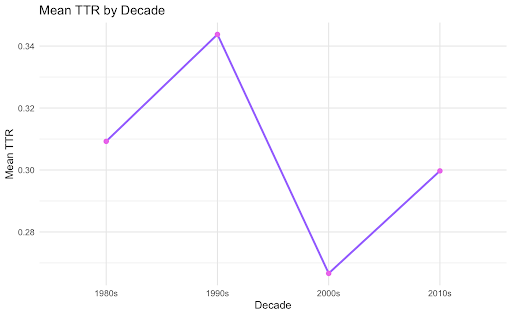
\includegraphics{images/mean_ttr.png}

}

\caption{Mean Type-Token Ratio by Decade}

\end{figure}%

A cursory inspection shows that the 1990s have a higher mean TTR while
the 2000s have a lower mean TTR relative to the 80s and 2010s.~To test
whether the apparent difference in TTR is statistically significant, we
decided to create a simple linear model.

\begin{figure}[H]

{\centering 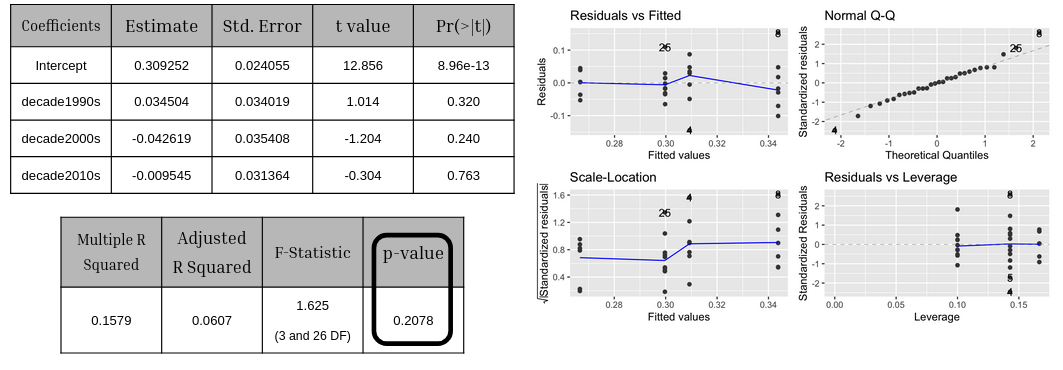
\includegraphics{images/Screenshot 2025-03-21 at 16-45-10 STATS 133 Are Romcoms Dead - Google Slides.png}

}

\caption{Linear Model and Assumption Tests}

\end{figure}%

To test whether the apparent difference in TTR is statistically
significant, we decided to create a simple linear model. Our model
followed the linearity assumptions, and none of the predictors were
significant, with the overall model itself not being significant. This
indicates that each decade's Mean TTR are actually not statistically
different. We can interpret this as meaning there is no real change in
the lexical diversity across decades.

Next, we looked at the most frequent words in each decade, creating
barplots and word clouds for each decade.

\textbf{Insert word cloud figure here}

There ``I'm'' is the most common word in all of the decades, followed by
``yeah'' (in all except the 90s).~Other shared common words include
really, time, day, night, talk, and gonna. This overlap of the most
common words in each decade supports the findings from lexical
diversity: so far, despite being from different eras, it seems that the
language of the rom-coms appears to remain very similar.

\textbf{Insert bigrams and trigrams here} and also include text
explanation of what they mean

\subsection{Sentiment Analysis}\label{sentiment-analysis}

The next technique applied was sentiment analysis, using
\citet{pang2008opinion} as a reference.

The AFINN Sentiment Score was employed for this dataset, which is a
lexicon that gives a score ranging from -5 to 5 for each word. Negative
scores indicate a negative sentiment while positive scores indicate a
positive sentiment. The graph below reveals the average AFINN sentiment
score per movie and by decade. All average scores are negative,
indicating there are more negatively rated words than positive in each
movie. Also, the scores vary greatly per movie. However, each decade is
relatively similar at around -0.5, except for the 2000s, which is at
-0.61.~

\begin{figure}[H]

{\centering 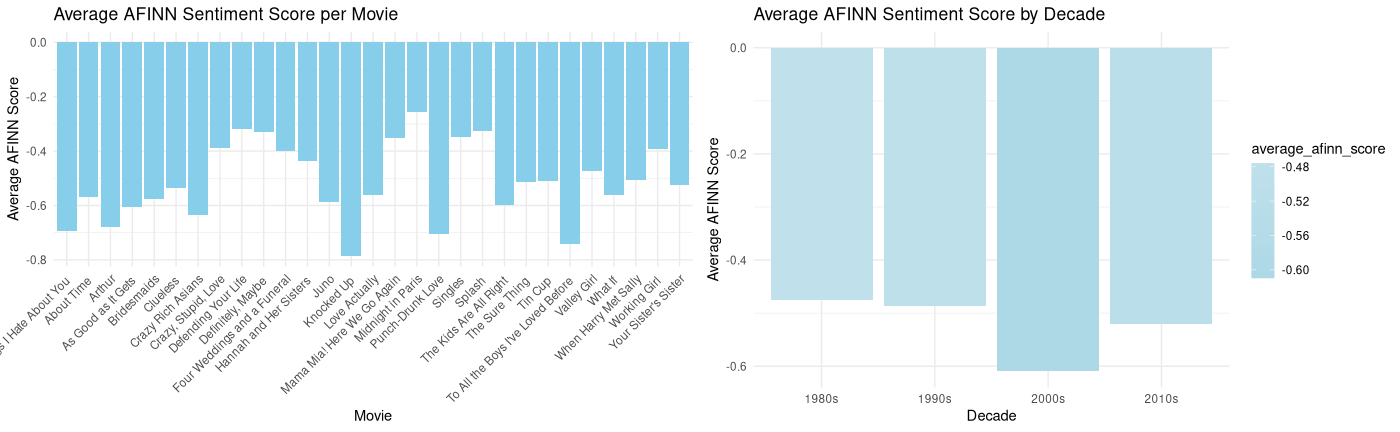
\includegraphics{images/avg_afinn-imageonline.co-merged.png}

}

\caption{Average AFINN scores for Movie and Decade}

\end{figure}%

Further analysis was done where the AFINN sentiment score was again
organized by movie and by decade. However, the scores were weighted by
TF-IDF, which evaluates how important a word is. Words with a higher
TF-IDF mean that the term is frequent in the specific document and rare
across the collection of documents. In the graph below, it is
interesting to note that by decade, the scores are vastly different when
compared to the graph above. When weighted by TF-IDF, the 1990s had the
least negative score, and the 2010s had the most negative score. When
only taking the average score, the 1990s and 2010s were very similar.
This indicates that in these 2 decades, frequent and important words
impact the overall movie sentiment greatly.

\begin{figure}[H]

{\centering 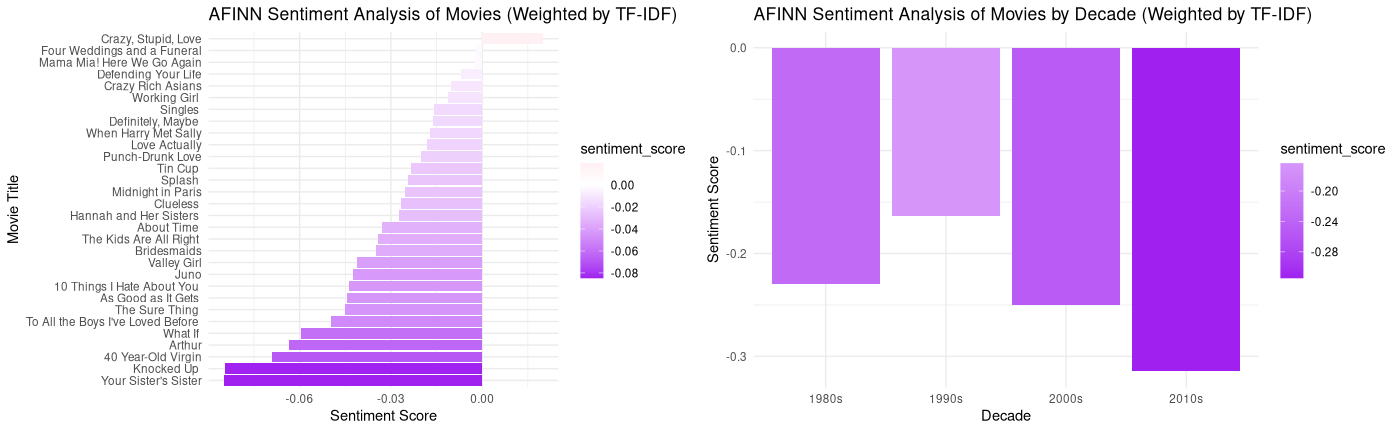
\includegraphics{images/decavgtdfif-imageonline.co-merged.png}

}

\caption{Average AFINN scores weighted by TF-IDF for Movies and Decade}

\end{figure}%

Lastly, the question of which emotions dominate was answered with the
NRC Lexicon. It associates words with 8 basic emotions. The bar graph
below reveals that, when words are weighted by TF-IDF, fear and trust
are the 2 most common emotions overall and by decade, with trust always
being the highest. This makes sense for romantic comedies, and most love
stories. This analysis did not reveal a significant change throughout
the decades. However, similarly to the AFINN sentiment score when
weighted by TF-IDF, the 1990s and 2010s show higher scores than the
other decades. This may mean that in these 2 decades, the important and
frequent words impact words of all emotions more than in the 1980s and
2000s.

\begin{figure}[H]

{\centering 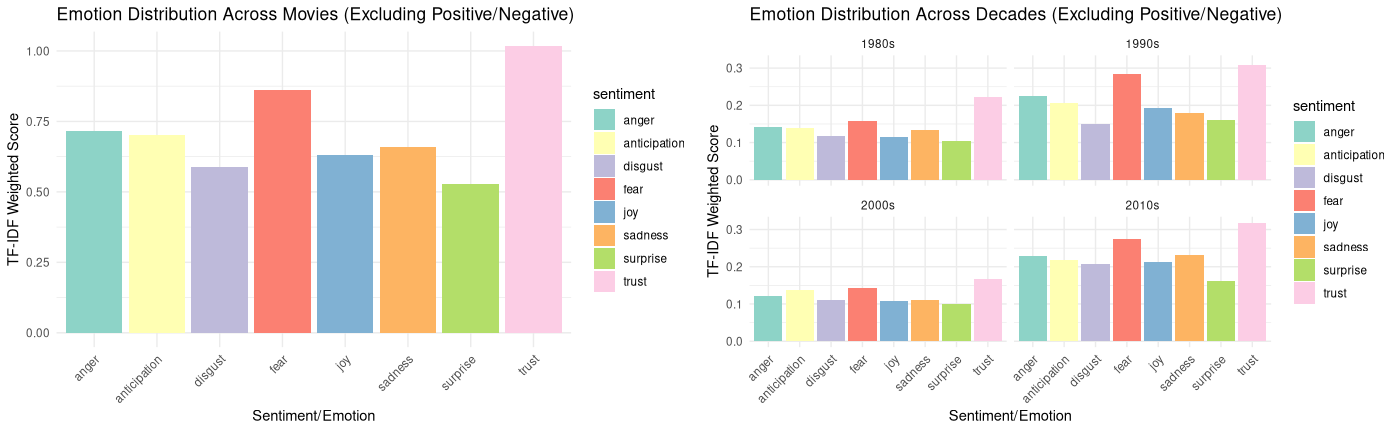
\includegraphics{images/nrc2-imageonline.co-merged.png}

}

\caption{Emotional Distribution by Movie and Decade}

\end{figure}%

\subsection{Clustering}\label{clustering}

K-means, Density-based, and Hierarchical clustering were all evaluated
on this dataset. While it is easy to see 3 separate groups of clusters
in all graphs, there are no patterns related to the decade group,
meaning that the movies are not able to be separated by decade. The
projected 2 dimensions indicate some kind of similarity amongst those in
the same cluster, but the decade labels are far from corresponding. This
indicates that though there may be factors that are able to cluster the
movies by similarity, these factors are not indicative of and do not
have any relation with the decade of movie production.

\begin{figure}[H]

{\centering 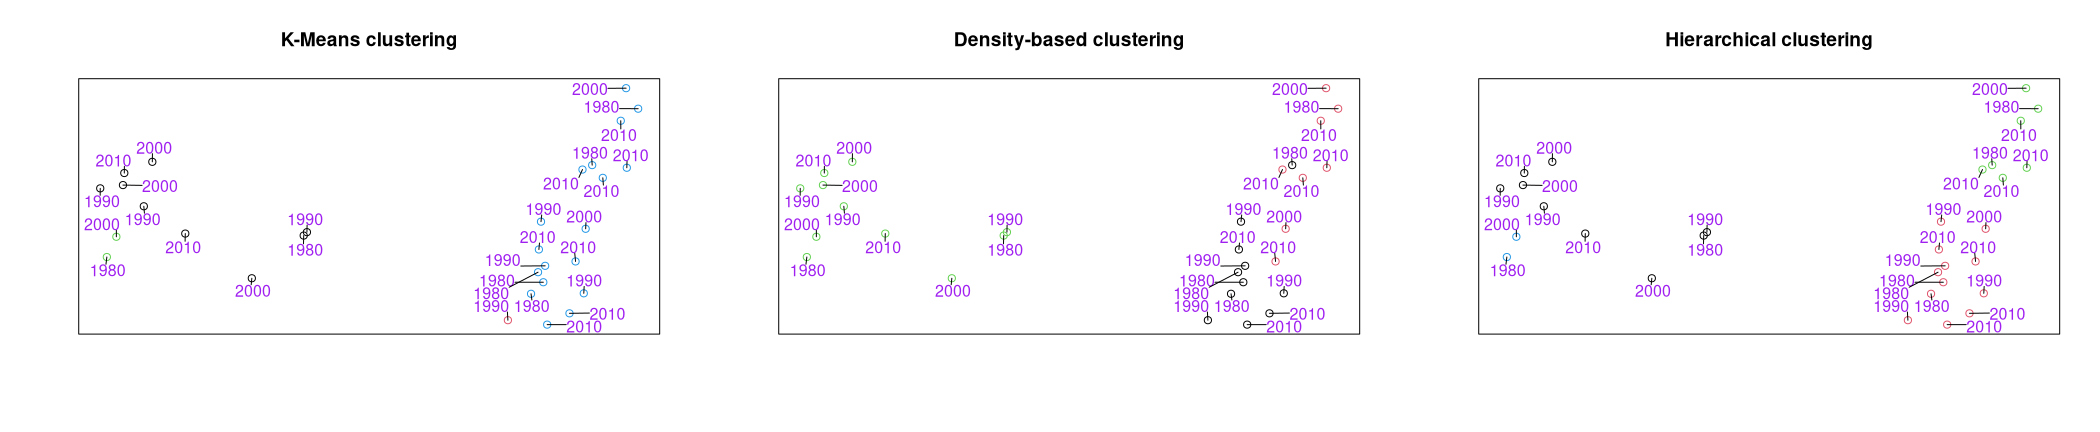
\includegraphics{images/hier-imageonline.co-merged.png}

}

\caption{Clustering Movies}

\end{figure}%

\subsection{Topic Modeling}\label{topic-modeling}

In order to see if the different decade groups could be differentiated
by topics, Latent Dirichlet Allocation (LDA) from \citet{ldapaper} was
utilized with a k value of 4. This essentially allocates each topic to
one of the 4 different movie decade groups. The most common words in
each of these groups are seen below.

\begin{figure}[H]

{\centering 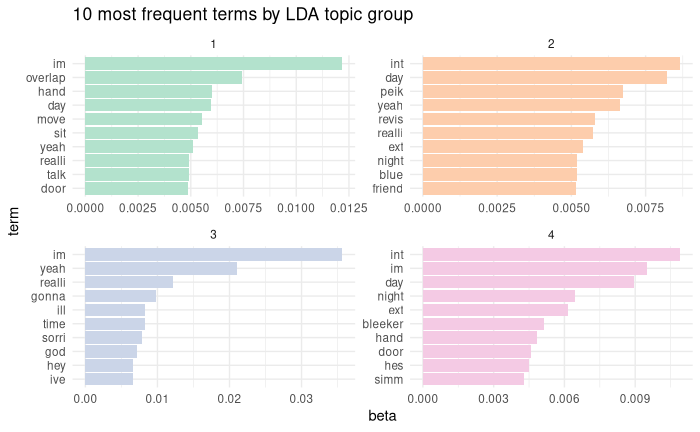
\includegraphics{images/freqLDA.png}

}

\caption{Most frequent terms by topic group}

\end{figure}%

From this alone, the words amongst different topics remain similar and
seem to indicate that the topics are not well separated. This is further
explored with a box plot of the gamma values from the LDA.

\begin{figure}[H]

{\centering 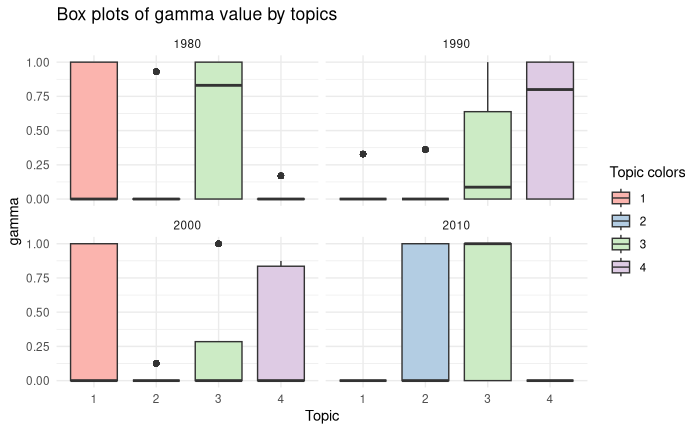
\includegraphics{images/boxplottopic.png}

}

\caption{Gamma boxplot by topic}

\end{figure}%

The boxplot reinforces that the topic modeling procedure was unable to
produce meaningful topic separation at the given k value of 4. Each plot
by decade group has multiple topic groups with large gamma values,
indicating that there is no direct relationship between a single topic
group and a single decade value. With this knowledge, we then attempt to
find the true topic separation within the movie data.

\begin{figure}[H]

{\centering 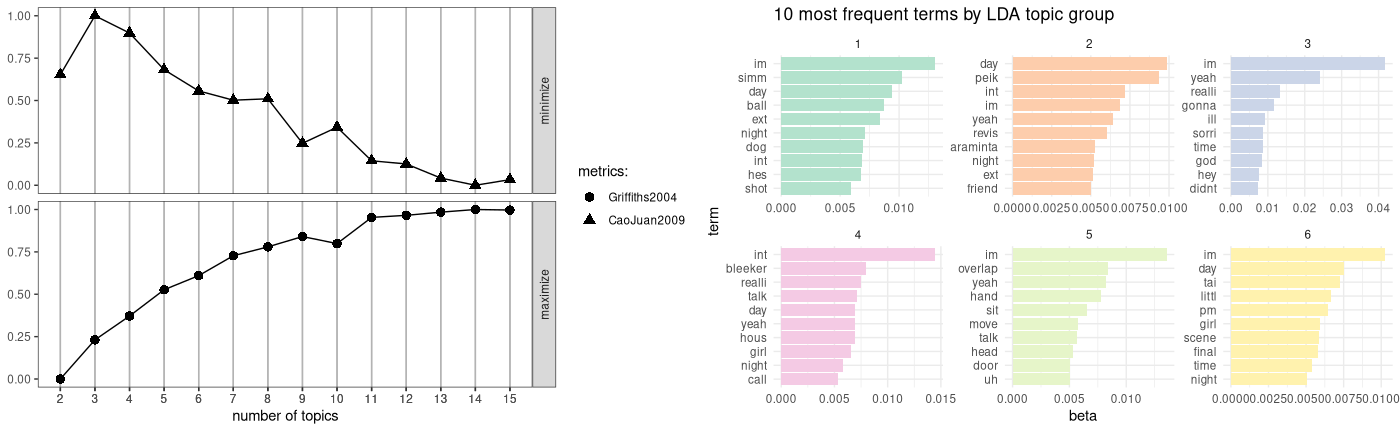
\includegraphics{images/lda6-imageonline.co-merged.png}

}

\caption{LDA tuning and topic designation}

\end{figure}%

Using the metrics Griffiths2004 and CaoJuan2009 from \citet{ldatuning}
as well as local experimentation, the chosen k value was 6. Once more,
from looking at the top terms, we can see similarity between topic
groups. However, there is a notable difference in unique terms for each
topic group, indicating that the topics are separated more here. For
these 6 topics, we then look at the document association with each of
the 6 topics.

\subsection{LLM Integration and
Prediction}\label{llm-integration-and-prediction}

Before this, we prompt ChatGPT to label each topic based on its most
frequent terms. The produced labels are: Golf Game, Social Gathering,
Emotional Conversation, Home Interaction, Everyday Moments, Christmas
Reflection.

\begin{figure}[H]

{\centering 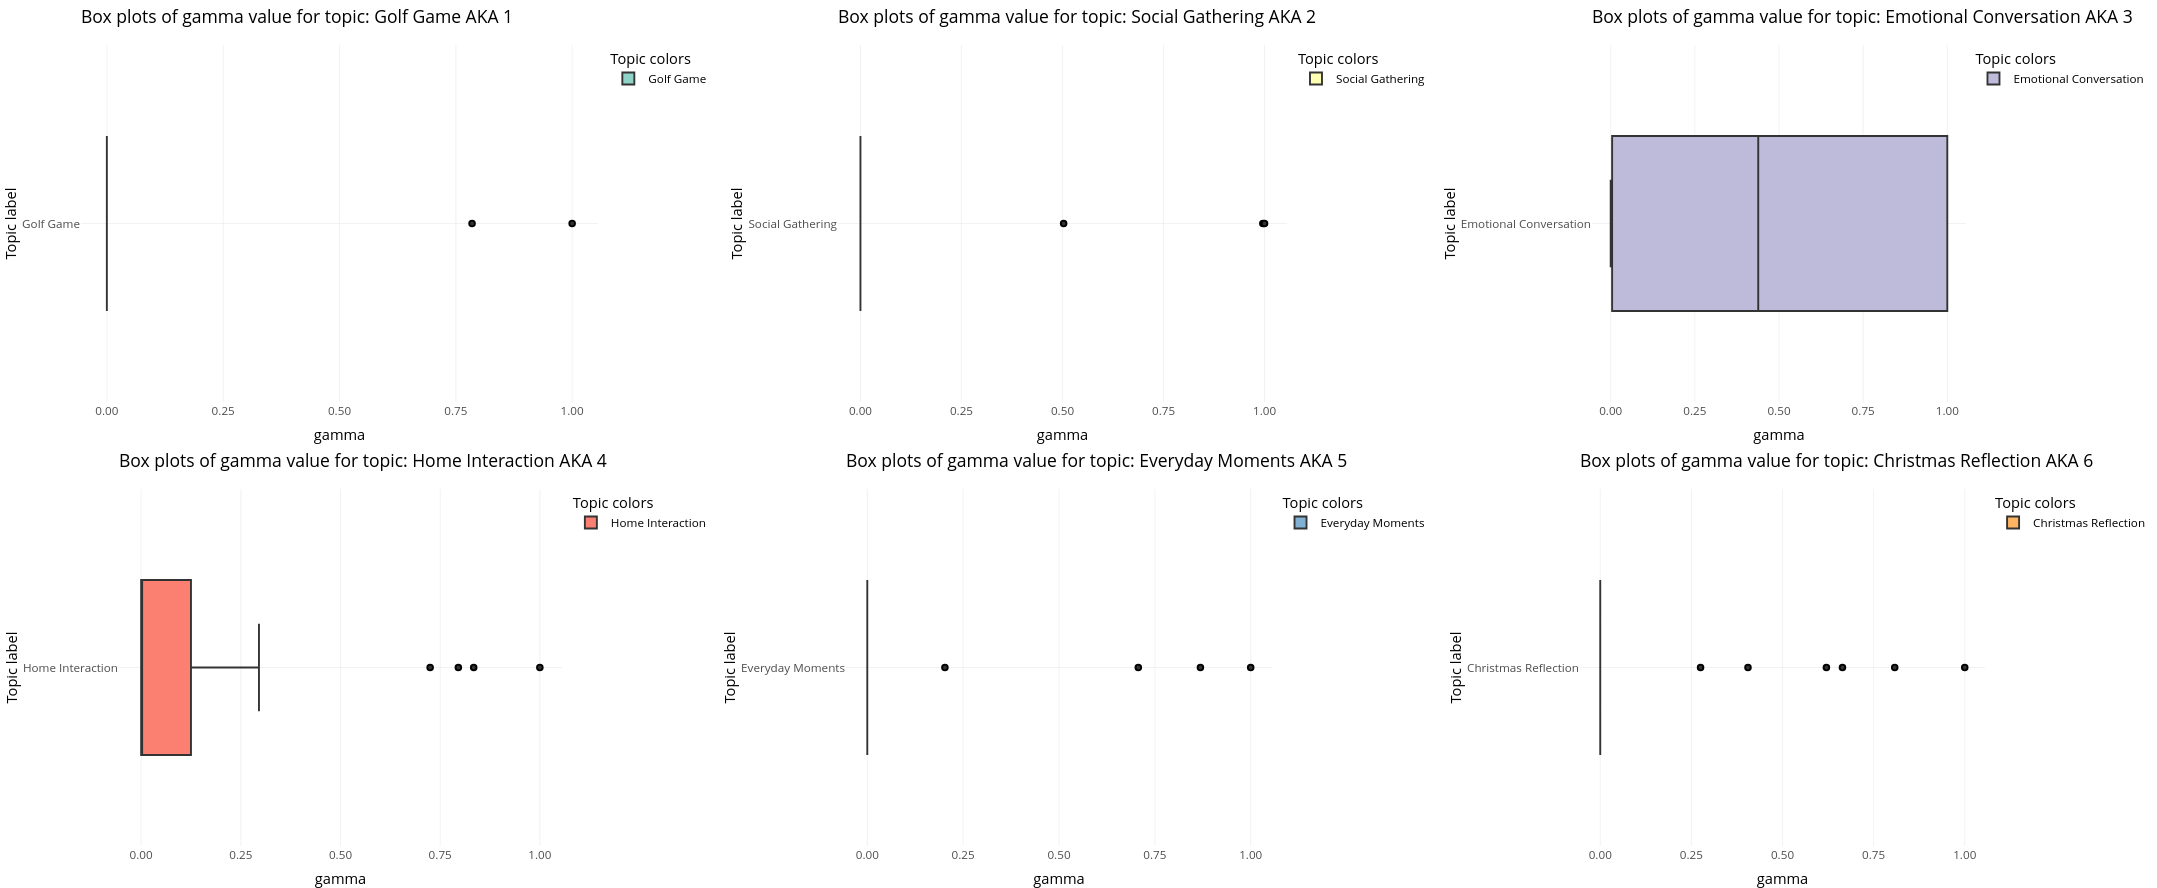
\includegraphics{images/top_topics_combined.png}

}

\caption{Gamma boxplots per labeled topic}

\end{figure}%

From these gamma boxplots, we can see the only topic with association
with a majority of the documents is the emotional conversation topic.
Thus, the documents themselves do not have an association with any other
specific topics.

With all of this, we aim to create a prediction model to classify the
decade of a movie based on its text content as features. In order to do
this, we incorporate two different methods. First, we create a more
traditional model with a Random Forest classifier. Then we use a
fine-tuned LLM to predict the decade label, using supplemental data for
the fine-tuning process and using two different ways of loading in our
data we want to make predictions on.

After using a 70-30 split between training and test data for the Random
Forest, we make our train and test predictions and produce the following
confusion matrices as well as a variable importance plot for the model
itself.

\begin{figure}[H]

{\centering 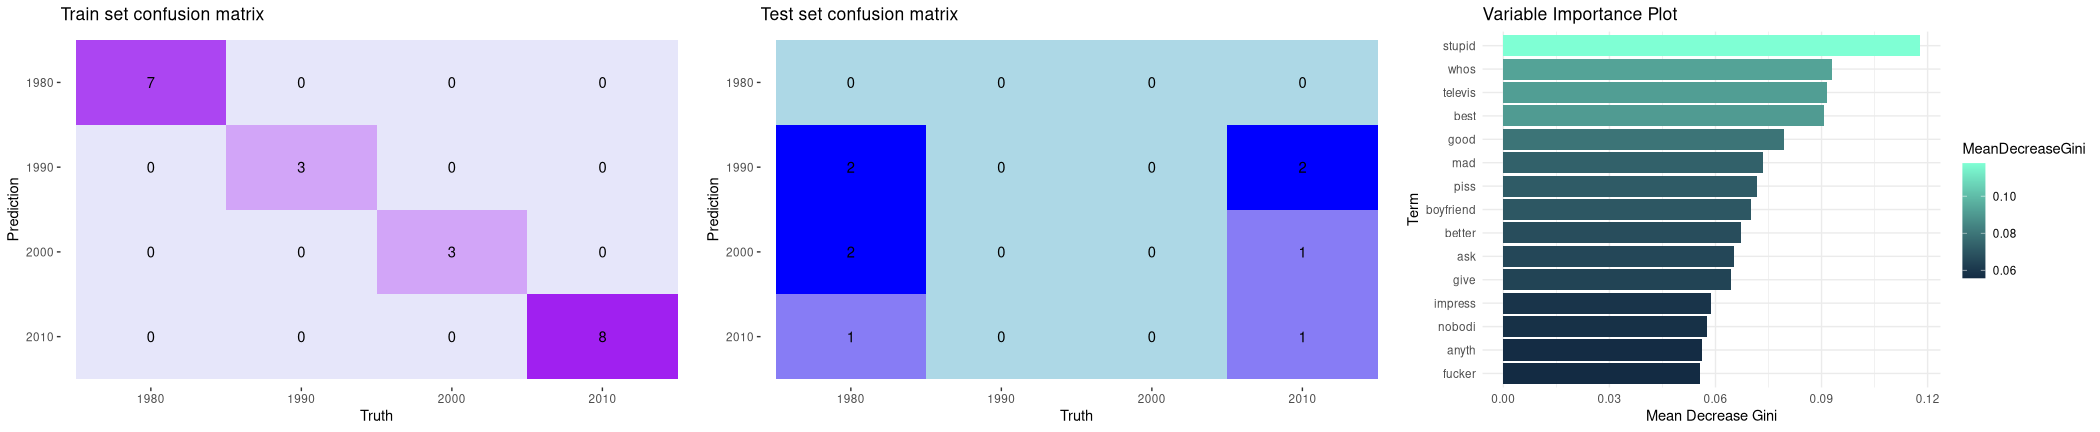
\includegraphics{images/rf_imp-imageonline.co-merged.png}

}

\caption{Random Forest Confusion Matrices and Variable Importance}

\end{figure}%

The training confusion matrix reports an accuracy of 100\%, but the
testing confusion matrix shows an accuracy of only 11.11\%. This
disparity in prediction indicates that the decade cannot be easily
predicted for a movie when using its text as the features. In this test
set, only one predicted case was classified correctly. As a result, we
turn to the LLM in order to use its contextual understanding and pattern
recognition capabilities to improve the accuracy of our decade class
predictions.~

We use two methods of loading in the training data after the fine-tuning
process has been completed. We first use chunking and weighting, which
breaks up each movie's text into chunks of 512 tokens and predicts the
class of each chunk before using a weighted average to assign an overall
class to a movie based on its chunks. The second method used is that of
truncation, in which the first 512 tokens are given for each movie and
classification is based on that input. The confusion matrices from
prediction are given below.

\begin{figure}[H]

{\centering 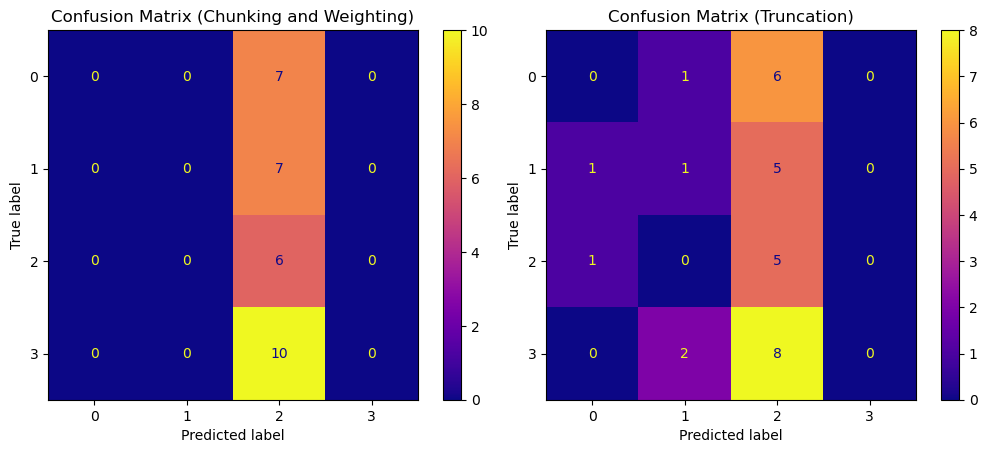
\includegraphics{images/trunc_llm-imageonline.co-merged.png}

}

\caption{LLM prediction confusion matrices}

\end{figure}%

As shown in each plot, both methods result in a test accuracy of 20\%.
However, the chunking and weighting approach predicts label 2,
corresponding to the 2000s decade, for each movie. On the other hand,
the truncation approach gives variety in prediction, though ultimately
only resulting in the same prediction accuracy. Of the two, the
truncation based prediction is the most promising. Ultimately, we
conclude that even with the utilization of LLMs, the decade of the movie
is hard to discern from its text data.

\section{Conclusion}\label{conclusion}

Through the use of correlation analysis, sentiment analysis, clustering,
topic modeling, and various forms of prediction, we uncovered insights
about the movie data that allowed us to learn more about each decade of
romantic comedies. Despite this, the additional data was not enough to
reliably differentiate movies across different eras. Thus, in terms of
numeric quantification, we were unable to uncover a significant
difference between the romantic comedies across the 4 eras. These
findings question the social perception of a decline in romantic
comedies, as the methods utilized in this paper present a story of
consistency and similarity. On the other hand, it should be noted that
perhaps the decline is a result of other processes and concepts not
covered in this analysis. Further work toward uncovering the reasoning
behind this perception may want to approach the questions from a
psychological point of view or consider other factors, such as the
acting of a movie, that were not considered in this process.


\renewcommand\refname{References}
  \bibliography{bibliography.bib}



\end{document}
